\documentclass[border=5pt]{standalone}
\usepackage{tikz}
\usepackage{amsmath}
\usetikzlibrary{calc, positioning, arrows.meta}
\begin{document}
% Force at angle diagram
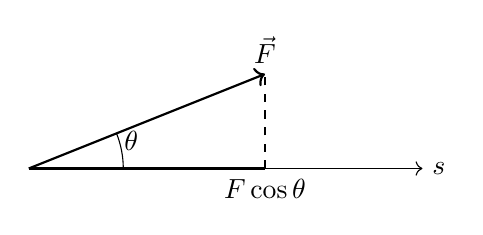
\begin{tikzpicture}[scale=1.0]
  % displacement axis
  \draw[->] (0,0) -- (5,0) node[right] {$s$};
  % force at angle
  \draw[->, thick] (0,0) -- (3,1.2) node[above] {$\vec{F}$};
  % parallel component
  \draw[thick] (0,0) -- (3,0) node[below] {$F\cos\theta$};

  \draw[dashed] (3,0) -- (3,1.2);
  % angle theta
  \draw (1.2,0) arc (0:21.8:1.2);
  \node at (1.3,0.35) {$\theta$};
\end{tikzpicture}

\vspace{1cm}

% Energy track with curve and incline
\begin{tikzpicture}[scale=0.8]
  % Point A (top of curve)
  \draw[thick] (0,3) node[above] {A} -- (0.5,2.5);
  \draw[thick] (0.5,2.5) to[out=-45, in=180] (2,0);

  % Point B (bottom)
  \fill (2,0) circle (2pt) node[below left] {B};

  % Rough horizontal BC
  \draw[thick] (2,0) -- (5,0);
  \fill (5,0) circle (2pt) node[below] {C};

  % Pattern for rough surface
  \foreach \x in {2.2,2.6,...,4.8}
    \draw (\x,-0.1) -- (\x+0.15,-0.25);

  % Smooth incline CD
  \draw[thick] (5,0) -- (7,1.15);
  \fill (7,1.15) circle (2pt) node[above right] {D};

  % Height annotation
  \draw[<->] (-0.5,0) -- (-0.5,3) node[midway, left] {$h_1=4$ m};

  % Distance annotation
  \draw[<->] (2,-0.7) -- (5,-0.7) node[midway, below] {$d=6$ m};

  % Angle annotation
  \draw (5.3,0) arc (0:30:0.3);
  \node at (5.6,0.15) {\small $\alpha$};
  \draw[dashed] (5,0) -- (6,0);

  % Ground
  \draw[thick] (-0.5,0) -- (2,0);
\end{tikzpicture}
\end{document}
